%%%%%%%%%%%%%%%%%%%%%%%%%%%%%%%%%%%%%%%%
%% MCM/ICM LaTeX Template %%
%% 2022 MCM/ICM           %%
%%%%%%%%%%%%%%%%%%%%%%%%%%%%%%%%%%%%%%%%
\documentclass[12pt]{article}
\usepackage{geometry}
\geometry{left=1.25in,right=1.25in,top=1in,bottom=1in}

%%%%%%%%%%%%%%%%%%%%%%%%%%%%%%%%%%%%%%%%
% Replace ABCDEF in the next line with your chosen problem
% and replace 1111111 with your Team Control Number
\newcommand{\Problem}{A}
\newcommand{\Team}{mby}
%%%%%%%%%%%%%%%%%%%%%%%%%%%%%%%%%%%%%%%%

\usepackage{newtxtext}
\usepackage{amsmath,amssymb,amsthm}
\usepackage{newtxmath} % must come after amsXXX

\usepackage{ctex}    %调用中文宏包
\usepackage{cite}
\usepackage{graphicx}%图片头文件
\usepackage{xcolor}
\usepackage{fancyhdr}
\usepackage{float}
\usepackage{booktabs}
\usepackage{lastpage}
\usepackage{multirow}
\usepackage{caption}

\usepackage{diagbox}
\usepackage{listings}
\usepackage{fontspec}
\usepackage{verbatim}
\usepackage{float} %指定图片位置
%\usepackage{subfigure}%并排子图 共享标题 有子标题
\usepackage{subcaption}
\usepackage{makecell}
%\usepackage{indentfirst}
\lhead{信号与系统2022- \Team}
\rhead{}
\cfoot{}

\newtheorem{theorem}{Theorem}
\newtheorem{corollary}[theorem]{Corollary}
\newtheorem{lemma}[theorem]{Lemma}
\newtheorem{definition}{Definition}

\begin{document}
\graphicspath{{images}}  % Place your graphic files in the same directory as your main document
\DeclareGraphicsExtensions{.pdf, .jpg, .tif, .png, .webp}
\thispagestyle{empty}
\vspace*{-16ex}
%\centerline{\begin{tabular}{*3{c}}

%%%%%%%%%%% Begin Summary %%%%%%%%%%%
% Enter your summary here replacing the (red) text
% Replace the text from here ...
%\begin{center}
    \section*{Summary}
\end{center}



\section*{Keywords} %%%小写

% to here
%%%%%%%%%%% End Summary %%%%%%%%%%%
\setlength{\headheight}{15pt}
%\clearpage
%%%%%%%%%%%%%%%%设置目录%%%%%%%%%%%%%%
\pagestyle{fancy}
% Uncomment the next line to generate a Table of Contents
\tableofcontents 
%\tableofcontents
\setcounter{page}{1}
\rhead{Page \thepage\ of \pageref{LastPage}}
%%%%%%%%%%%%%%%%%%%%%%%%%%%%%%

%%%%%%%%%%%%%%%%开始正文%%%%%%%%%%%%%%
\newpage
\section{设计名称}
去除干扰蜂鸣音
\section{实验目的}
\indent 掌握信号时频域分析方法,正确理解采样定理,准确理解滤波器的概念。


\section{设计要求}
\indent 提供一个包含某人说话语音片段的声音文件( buzz.wav ),但该语音信号被一个包含有几个谐波分量的蜂鸣信号干扰了。
\begin{itemize}
    \item [\textbf{1.}] 用Matlab的wavread命令读取该声音文件。注意,该命令可以同时得到声音文件的采样率和采样位宽,请查阅 Matlab 的帮助文件。
    \item [\textbf{2.}] 用快速傅立叶变换(FFT)计算并画出声音信号的频谱,列写出蜂鸣信号的谐波频率。
    \item [\textbf{3.}] 思考如何将这些蜂鸣音去除?将去除了蜂鸣音的语音片段播放出来,仔细聆听并写下语音片段中人物所说的话。注意:由于只能播放实信号,因此记得提取信号的实部。
\end{itemize} 

\section*{代码附录}

\definecolor{vgreen}{RGB}{104,180,104}
\definecolor{vblue}{RGB}{49,49,255}
\definecolor{vorange}{RGB}{255,143,102}
\lstdefinestyle{verilog-style}
{
    language=Verilog,
    basicstyle=\ttfamily,
    keywordstyle=\color{vblue},
    identifierstyle=\color{black},
    commentstyle=\color{vgreen},
    numbers=left,
    frame=shadowbox,
    breaklines=true, 
    numberstyle={\tiny \color{black}},
    numbersep=10pt,
    tabsize=8
}
\begin{lstlisting}[
    style={verilog-style}]
//1:顶层模块===============================================
 module top_module(
  input clk,
  input start,    
  input reset, 
  input key0,key1,key2,key3,
  output row,
  output [3:0]led,
  output [5:0]dig,
  output [7:0]seg,
  output beep,
  output [4:0]led_b);
    assign row=1'b0;
    wire clk_1k;
    wire clk_1s;
    wire clk_20ms;

  fenpin u1(.clk(clk),
         .clk_1k(clk_1k),
         .clk1sout(clk_1s),
         .clk_20ms(clk_20ms));
         
         wire k0;
         wire k1;
         wire k2;
         wire k3;
  key_debounce u2(
         .clk(clk_20ms),
         .key_in(key0),
         .key_out(k0));
  key_debounce u3(
         .clk(clk_20ms),
         .key_in(key1),
         .key_out(k1));
  key_debounce u4(
         .clk(clk_20ms),
         .key_in(key2),
         .key_out(k2));
  key_debounce u5(
         .clk(clk_20ms),
         .key_in(key3),
         .key_out(k3));    
  wire [1:0]state;
  wire [1:0]floor;      
  operation u6(
         .clk(clk),
         .set(start),
         .reset(reset),
         .key0(k0),
         .key1(k1),
         .key2(k2),
         .key3(k3),
         .led(led),
         .state(state),
         .floor(floor)); 
  display u7(
         .floor(floor),
         .state(state),
         .clk(clk_1k),
         .seg(seg),
         .clk_1s(clk_1s),
         .led_b(led_b),
         .dig(dig)); 
  beep u8(
         .clk(clk),
         .state(state),
         .floor(floor),
         .beep(beep));                                          
endmodule

//2.分频器===============================================
module fenpin(
    input clk,clr,
    output reg clk_1k=0,  //1kHz信号
    output reg clk1sout=0,//1Hz信号
    output reg clk_20ms=0,//50Hz信号
    integer    clk1s_cnt=0
    );
 reg[24:0] cnt=0;
 always @ (posedge clk)//分频得到1kHz信号
    begin
      if (cnt==25000)
        begin
           clk_1k=~clk_1k; cnt=0;
         end
      else  cnt=cnt+1;
    end

reg [31:0] temp = 0;
always@(posedge clk)//分频得到50Hz信号
    begin
      if(temp == 999999)
      begin
            temp <= 0;clk_20ms <= ~clk_20ms;
      end
      else  temp <= temp+1;
      end
 
 always@(posedge clk)//分频得到1Hz信号
 begin    
    if(clr)    
    begin   
           clk1s_cnt<=0; clk1sout<=0;  
    end 
    else  if(clk1s_cnt==24999999) 
    	begin
     	   clk1s_cnt<=0;clk1sout<=~clk1sout;
     	end
    else   clk1s_cnt<=clk1s_cnt+1;
 end
endmodule

//3.按键消抖模块=====================================
module key_debounce(
    input key_in,
    input clk,
    output key_out);
    reg  btn0=0;
    reg  btn1=0;
    reg  btn2=0;

always@(posedge clk)
  begin
    btn0<=key_in;
    btn1<=btn0;
    btn2<=btn1;
  end
 
assign key_out=((btn0&btn1)&(~btn2) | (btn0&btn1&btn2) | ((~btn0)&btn1&btn2));
endmodule

//4.状态控制模块=======================================
module operation(
    input clk,
    input set,
    input reset,
    input key0,
    input key1,
    input key2,
    input key3,
    output reg [3:0]led=0,//指示灯
    output reg [1:0]state=0,//0待机状态;1上行;2下行
    output reg [1:0]floor=1  //1一楼;2二楼 
	);
    reg [27:0]cnt=0; 
    reg [27:0]clk_count=0;
    reg k0=0;
    reg k1=0;
    reg k2=0;
    reg k3=0; 
    reg [1:0] first=0; 
always@(posedge clk)
  begin
    if(!reset)//复位开关被拨回
       begin
           if(floor==2)//如果电梯在2楼,则运行五秒后回到一楼
             if(clk_count==249999999) //5s计时
             begin            
                clk_count=0;  
                floor=1;    //1楼                  
                state=0;    //待机状态       
                led=4'b0000;//指示灯不亮
              end
             else 
             begin 
                clk_count=clk_count+1;
                state=2;    //下行状态
                led=4'b0000;//指示灯不亮
             end
       end
   else if(set)//复位开关未被拨下,且启动start有效
   begin
     if(led)//当led非0,即电梯处于运行状态时
       begin 
         if(clk_count==249999999)//5s计时 
          begin            
            clk_count=0;                        
            if(floor==1)  
                begin floor=floor+1; 
                end//计时五秒后从一楼切换到二楼
            else        
                begin floor=floor-1; 
                end//计时五秒后从二楼切换到一楼       
            
            //key3,key2接连被按下,到二楼后保持led2亮起,切换到下行状态
            if((k3&k2)&&first==1) 
                begin state=2;k3=0;k2=0;led[3]=0;first=0;
                end

            //key3,key0接连被按下,到二楼后保持led0亮起,切换到下行状态
            else if(k3&k0) 
                begin state=2;k3=0;k0=0;led[3]=0;
                end

            //key2,key3接连被按下,到一楼后保持led3亮起,切换到上行状态
            else if((k2&k3)&&first==2) 
                begin state=1;k2=0;k3=0;led[2]=0;first=0;
                end

            //key2,key1接连被按下,到一楼后保持led1亮起,切换到上行状态
            else if(k2&k1) 
                begin state=1;k2=0;k1=0;led[2]=0;
                end

            //回到待机状态
            else  
                begin state=0;led=4'b0000;k0=0;k1=0;k2=0;k3=0;
                end 
          end 

         else  clk_count=clk_count+1;
    //在运行过程中保持指示灯正常亮起,并且在按键在电梯运行过程中被按下时进行记录
     if(key2|k2)
        begin k2=1;k0=0;led[2]=1;
        end
     if(key0|k0) 
        begin k0=1;k2=0;led[0]=1;
        end
     if(key3|k3) 
        begin k3=1;k1=0;led[3]=1;
        end
     if(key1|k1) 
        begin k1=1;k3=0;led[1]=1;
        end
    end
        
    else if((key0)&&floor==2)  //当前在二楼,一楼按key0
            begin
                led[0]=1; 
                state=2; //下行                         
            end
                                
    else if((key1)&&floor==1)  //当前在一楼,二楼按key1
            begin
                led[1]=1;
                state=1;//上行
            end
     
    else if((key2)&&floor==2)  //当前在二楼 电梯内按下 
            begin
                led[2]=1;
                state=2; //下行
                k2=1;
                first=2;//用于表明key2先于key3被按下
            end 
                                 
    else if((key3)&&floor==1)  //当前在一楼 电梯内按上  
            begin
                led[3]=1;
                state=1; //上行 
                k3=1;
                first=1;//用于表明key3先于key2被按下
            end
        end
    end
endmodule

//5.译码显示及流水指示灯模块==========================

module display(
    input [1:0]floor,//楼层
    input [1:0]state,//状态
    input clk,
    input clk_1s,
    output reg [4:0] led_b=0,
    output reg [7:0] seg,
    output reg [5:0] dig
);
reg num=0;
	always@(posedge clk)
	begin
		if (num==1) num=0;
		else num=num+1;
	end
   //位选
	always@(num)
	begin	
		case(num)
		0:dig=6'b111110;
		1:dig=6'b111101;
		default: dig=0;
		endcase
	end
	
always@(posedge clk_1s or posedge state or negedge state)
begin
	if(state==0)
	    led_b[4:0]=5'b00000;
    else if (state ==1)//电梯处于上行状态
        begin
            if (led_b[4:0]==5'b00000)
                led_b[4:0]=5'b10000;
        else
                led_b[4:0]=led_b[4:0]>>1; 
    //向右移一位。10000-01000-00100-00010-00001-00000
        end
    else if (state ==2)//电梯处于下行状态
        begin
            if (led_b[4:0]==5'b00000)
                led_b[4:0]=5'b00001;//到了00000,下一个是00001
            else
                led_b[4:0]=led_b[4:0]<<1; 
    //向左移一位。00001-00010-00100-01000-10000-00000
        end
    else led_b[4:0]=5'b00000;
	end
	
//选择器,确定显示数据
reg [3:0] disp_data;
always@(num)
begin	
	case(num)
	0:disp_data=floor;
	1:disp_data=state+3'b011;//3待机 4上行 5下行
	default: disp_data=0;
	endcase
end	
//显示译码器
always@(disp_data)
	begin
		case(disp_data)
		4'h1: seg=8'h06;//1楼
		4'h2: seg=8'h5b;//2楼
		4'h3: seg=8'h40;//待机
		4'h4: seg=8'h01;//上行
		4'h5: seg=8'h08;//下行
		default: seg=0;
		endcase
	end
endmodule

//6.蜂鸣==================================
module beep(
    input clk,
    input [1:0]state,
    input [1:0]floor,
    output reg beep
    );  
    reg beep_n;//控制蜂鸣声时长
    reg [24:0] beep_cnt=0;
    reg [24:0] clk_500ms_cnt=0;
    reg [24:0] clk_500ms_cnt2=0;   
      always @ (posedge clk)
        begin 
            if(floor==1)
              begin
                clk_500ms_cnt2=0;
                if (clk_500ms_cnt==24999999)//计数0.5s,在此区间发出蜂鸣声
                    begin
                        beep_n=0;
                        clk_500ms_cnt=24999999;
                    end
                else if(clk_500ms_cnt!==24999999&&clk_500ms_cnt!==0)
                    begin
                        clk_500ms_cnt<=clk_500ms_cnt+1;
                        beep_n=1;
                    end  
                else if(clk_500ms_cnt==0)
                    begin
                        clk_500ms_cnt<=clk_500ms_cnt+1;
                        beep_n=0;
                    end
                end 
            else
                begin
                  clk_500ms_cnt=0;
                if (clk_500ms_cnt2==24999999)
                //计数0.5s,在此区间发出蜂鸣声
                    begin
                      beep_n=0;
                      clk_500ms_cnt2=24999999;
                    end
                else if(clk_500ms_cnt2!==24999999&&clk_500ms_cnt2!==0)
                     begin
                        clk_500ms_cnt2<=clk_500ms_cnt2+1;
                        beep_n=1;
                     end  
                else if(clk_500ms_cnt2==0)
                     begin
                        clk_500ms_cnt2<=clk_500ms_cnt2+1;
                        beep_n=0;
                     end
                end 

         if(beep_n==1)
             begin
               if(beep_cnt==49000)
               //向蜂鸣器输入一个约500Hz的脉冲,使蜂鸣器发声
                 begin
                  beep=~beep; 
                  beep_cnt=0;
                 end
                else
                  begin beep_cnt=beep_cnt+1;end 
              end    
         else
             begin
              beep=0;
              beep_cnt=0;          
             end          
    end     
endmodule

//约束文件======================================
set_property IOSTANDARD LVCMOS33 [get_ports {dig[5]}]
set_property IOSTANDARD LVCMOS33 [get_ports {dig[4]}]
set_property IOSTANDARD LVCMOS33 [get_ports {dig[3]}]
set_property IOSTANDARD LVCMOS33 [get_ports {dig[2]}]
set_property IOSTANDARD LVCMOS33 [get_ports {dig[1]}]
set_property IOSTANDARD LVCMOS33 [get_ports {dig[0]}]
set_property IOSTANDARD LVCMOS33 [get_ports {led[3]}]
set_property IOSTANDARD LVCMOS33 [get_ports {led[2]}]
set_property IOSTANDARD LVCMOS33 [get_ports {led[1]}]
set_property IOSTANDARD LVCMOS33 [get_ports {led[0]}]
set_property IOSTANDARD LVCMOS33 [get_ports {seg[7]}]
set_property IOSTANDARD LVCMOS33 [get_ports {seg[6]}]
set_property IOSTANDARD LVCMOS33 [get_ports {seg[5]}]
set_property IOSTANDARD LVCMOS33 [get_ports {seg[4]}]
set_property IOSTANDARD LVCMOS33 [get_ports {seg[3]}]
set_property IOSTANDARD LVCMOS33 [get_ports {seg[2]}]
set_property IOSTANDARD LVCMOS33 [get_ports {seg[1]}]
set_property IOSTANDARD LVCMOS33 [get_ports {seg[0]}]
set_property IOSTANDARD LVCMOS33 [get_ports beep]
set_property IOSTANDARD LVCMOS33 [get_ports clk]
set_property PACKAGE_PIN T5 [get_ports {led[3]}]
set_property PACKAGE_PIN R7 [get_ports {led[2]}]
set_property PACKAGE_PIN R8 [get_ports {led[1]}]
set_property PACKAGE_PIN P9 [get_ports {led[0]}]
set_property PACKAGE_PIN D4 [get_ports clk]
set_property PACKAGE_PIN L2 [get_ports beep]
set_property PACKAGE_PIN N11 [get_ports {dig[5]}]
set_property PACKAGE_PIN N14 [get_ports {dig[4]}]
set_property PACKAGE_PIN N13 [get_ports {dig[3]}]
set_property PACKAGE_PIN M12 [get_ports {dig[2]}]
set_property PACKAGE_PIN H13 [get_ports {dig[1]}]
set_property PACKAGE_PIN G12 [get_ports {dig[0]}]
set_property PACKAGE_PIN L13 [get_ports {seg[7]}]
set_property PACKAGE_PIN M14 [get_ports {seg[6]}]
set_property PACKAGE_PIN P13 [get_ports {seg[5]}]
set_property PACKAGE_PIN K12 [get_ports {seg[4]}]
set_property IOSTANDARD LVCMOS33 [get_ports reset]
set_property IOSTANDARD LVCMOS33 [get_ports start]
set_property PACKAGE_PIN F3 [get_ports reset]
set_property PACKAGE_PIN T9 [get_ports start]
set_property PACKAGE_PIN K13 [get_ports {seg[3]}]
set_property PACKAGE_PIN L14 [get_ports {seg[2]}]
set_property PACKAGE_PIN N12 [get_ports {seg[1]}]
set_property PACKAGE_PIN P11 [get_ports {seg[0]}]
set_property PACKAGE_PIN K3 [get_ports row]
set_property IOSTANDARD LVCMOS33 [get_ports row]
set_property IOSTANDARD LVCMOS33 [get_ports key0]
set_property IOSTANDARD LVCMOS33 [get_ports key1]
set_property IOSTANDARD LVCMOS33 [get_ports key2]
set_property IOSTANDARD LVCMOS33 [get_ports key3]
set_property PACKAGE_PIN R12 [get_ports key0]
set_property PACKAGE_PIN T12 [get_ports key1]
set_property PACKAGE_PIN R11 [get_ports key2]
set_property PACKAGE_PIN T10 [get_ports key3]
set_property IOSTANDARD LVCMOS33 [get_ports {led_b[4]}]
set_property IOSTANDARD LVCMOS33 [get_ports {led_b[3]}]
set_property IOSTANDARD LVCMOS33 [get_ports {led_b[2]}]
set_property IOSTANDARD LVCMOS33 [get_ports {led_b[1]}]
set_property IOSTANDARD LVCMOS33 [get_ports {led_b[0]}]
set_property PACKAGE_PIN T2 [get_ports {led_b[0]}]
set_property PACKAGE_PIN R1 [get_ports {led_b[1]}]
set_property PACKAGE_PIN G5 [get_ports {led_b[2]}]
set_property PACKAGE_PIN H3 [get_ports {led_b[3]}]
set_property PACKAGE_PIN E3 [get_ports {led_b[4]}]

\end{lstlisting}   
    

\section{步骤分析}
$\bullet$做音频信号时域图,由于蜂鸣干扰,时域图像如下:
\begin{figure}[H]
    \centering
    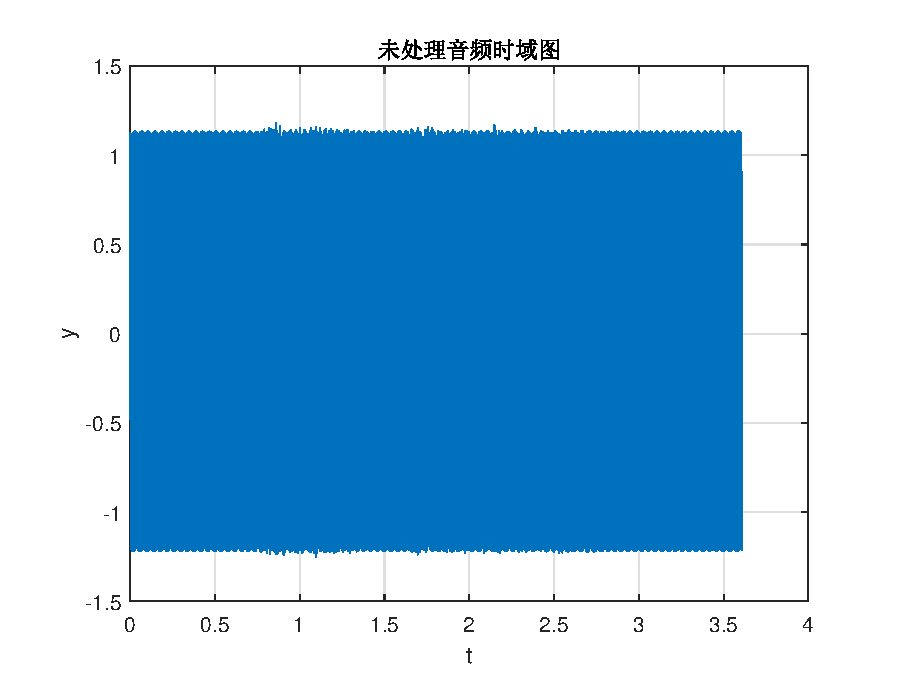
\includegraphics[width=8cm]{un-pict.eps}
    \caption{原音频信号时域图 }
\end{figure}
$\bullet$做音频信号频域图,并根据频域图像标记噪声频谱。\textit{此类噪声为单音噪声}\\\textit{单音噪声的消除首先考虑以某一幅度标准为限制,高于此幅度的进行滤除}
\begin{figure}[H]
    \centering
    \subcaptionbox{原音频信号频域图}{
        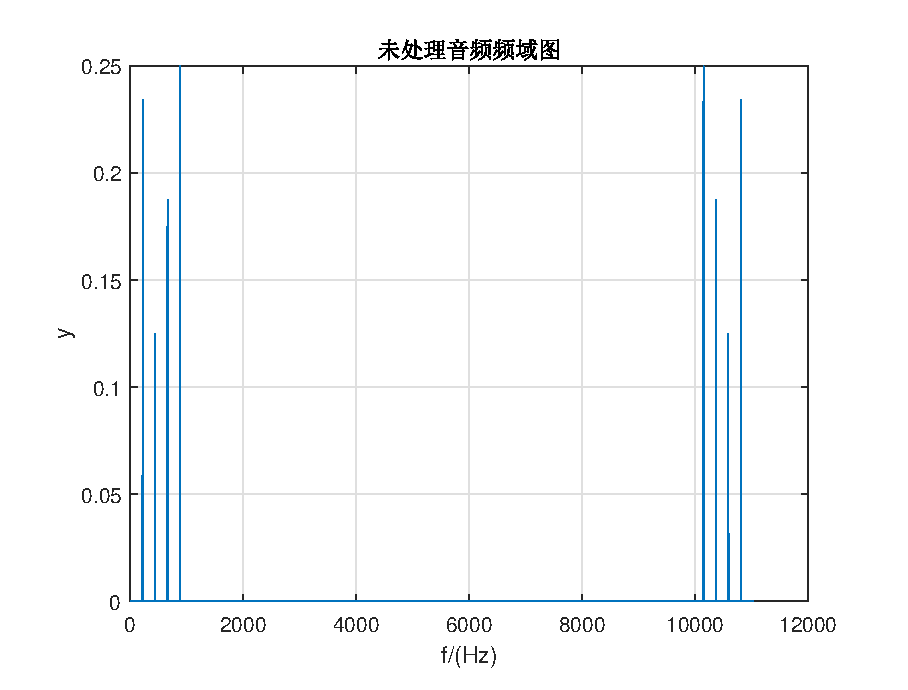
\includegraphics[width=11cm]{un-picf1.eps}	
    }
    \hfill 
    \subcaptionbox{原音频信号频域图-【标记噪声】}{
        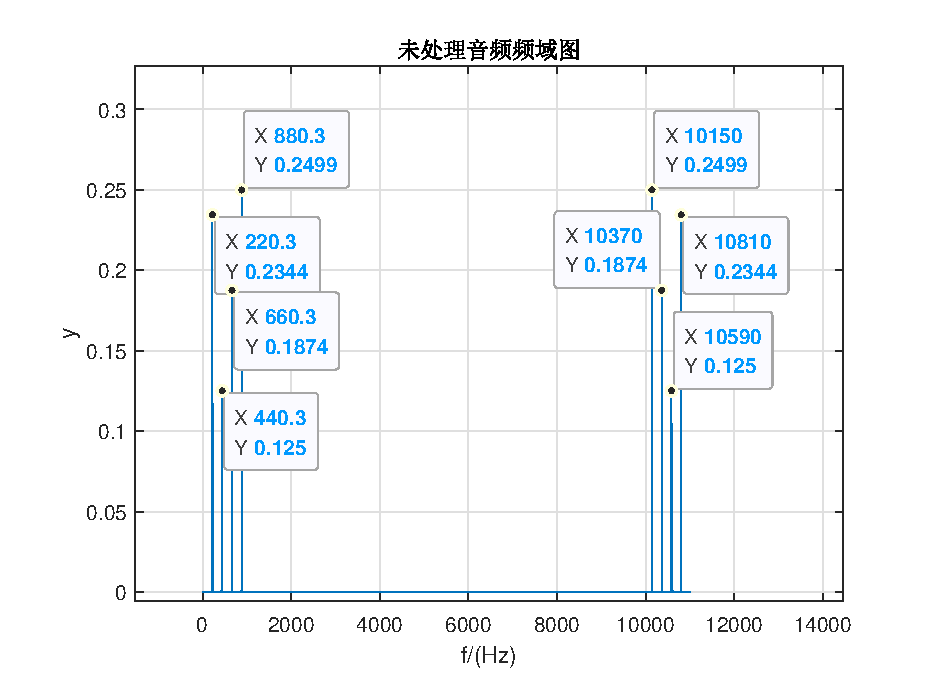
\includegraphics[width=11cm]{un-picf.eps}	
    }
    \caption{原音频信号频域图}
\end{figure}
\newpage
$\bullet$对音频信号进行初步处理。\textit{标记点y值:即为单音噪声滤除的幅度标准;标记点x值可判断出滤波器的上下限截止频率}\\
\indent 此时,已经可以消除绝大部分蜂鸣噪声,并辨析出该段音频在播放:\textit{‘这里是电子科技大学’}。

\begin{figure}[H]
    \centering
    \subcaptionbox{频域图}{
        \includegraphics[width=11cm]{af-picf.eps}	
    }
    \hfill 
    \subcaptionbox{时域图}{
        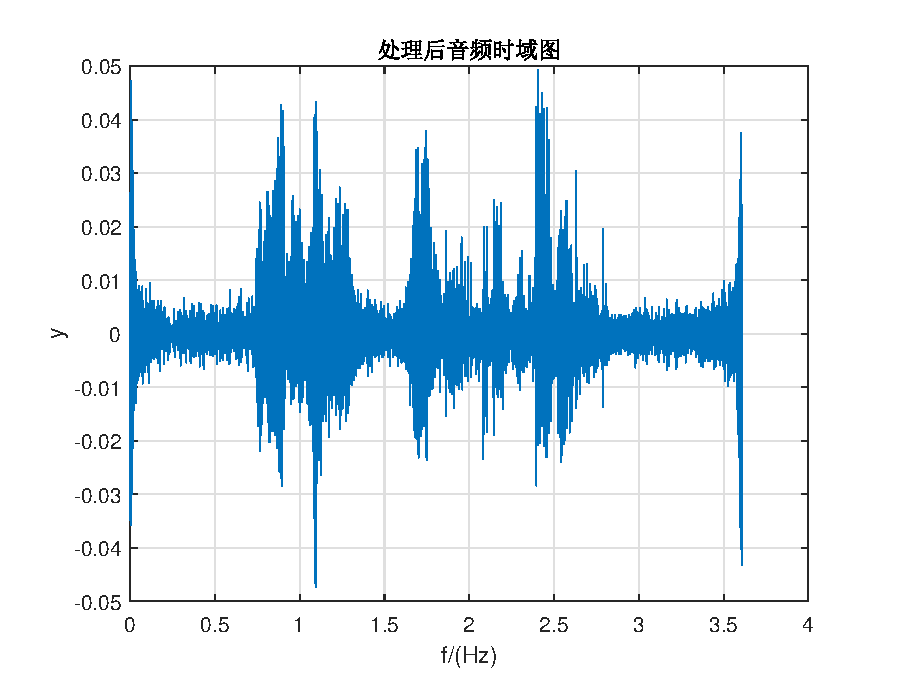
\includegraphics[width=11cm]{af-pict1.0.eps}	
    }
    \caption{一次处理后音频信号频域域图}
\end{figure}
\newpage
$\bullet$但是,第一步处理后听到处理音频仍伴随着持续低噪声,考虑使用带通滤波器直接去除双边频域信号.观测时域图也可发现,时域音频的‘毛刺’明显减少\\
\indent 此时持续低噪声明显消失,但此时人声听起来‘失真’,效果稍显不佳。\textit{(与初步处理音频相比更不像真人说话的效果,可以认为处理效果较为不佳)}

\begin{figure}[H]
    \centering
    \subcaptionbox{处理音频信号频域图}{
        \includegraphics[width=11cm]{af-picf0.eps}	
    }
    \hfill 
    \subcaptionbox{处理音频信号时域图}{
        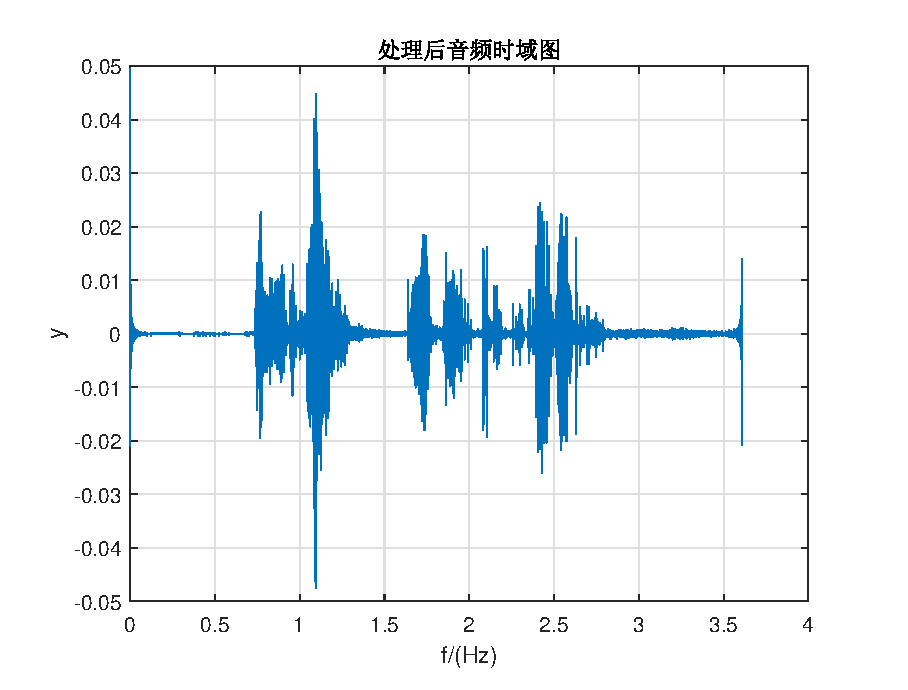
\includegraphics[width=11cm]{af-pict0.0.eps}	
    }
    \caption{全部滤波处理后音频信号频域域图}
\end{figure}
\newpage
$\bullet$ 人声听起来‘失真’,会不会是因为被滤去的双侧信号中仍含有部分音频信息呢?\\
\indent 于是,取双侧信号进行频域、时域分析,声音处理后仍可勉强辨识出,男声:‘这里是电子科技大学’。\\
\indent 不过,此时人声清晰度明显不足,且伴有较大噪声。但是仍可从此次变换中得到双侧\textbf{信号仍包含重要信息不应该被简单置零}的结论。\\
\begin{figure}[H]
    \centering
    \subcaptionbox{频域图}{
        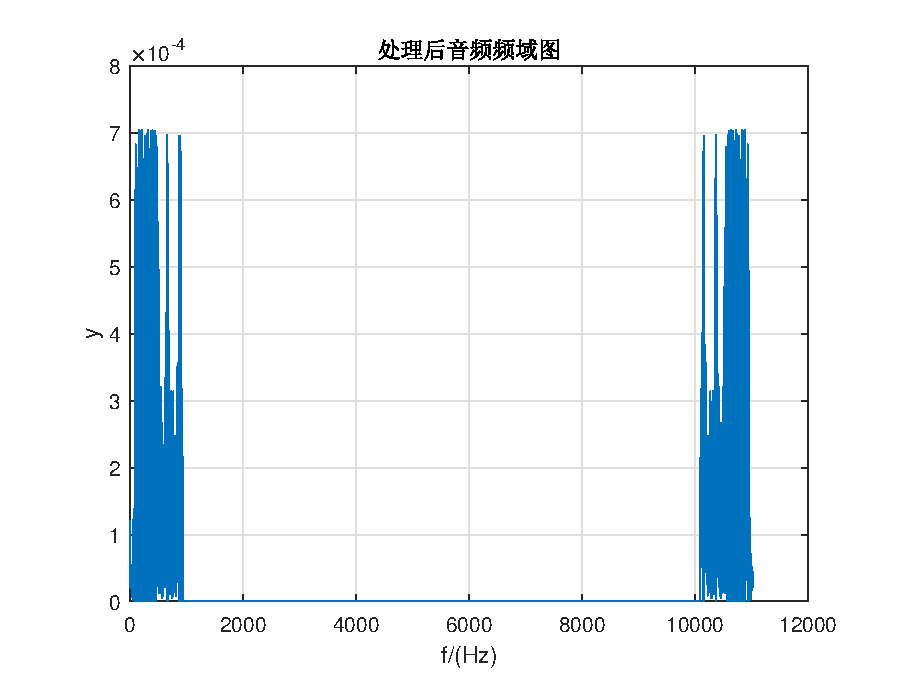
\includegraphics[width=10cm]{111.eps}	
    }
    \hfill 
    \subcaptionbox{时域图}{
        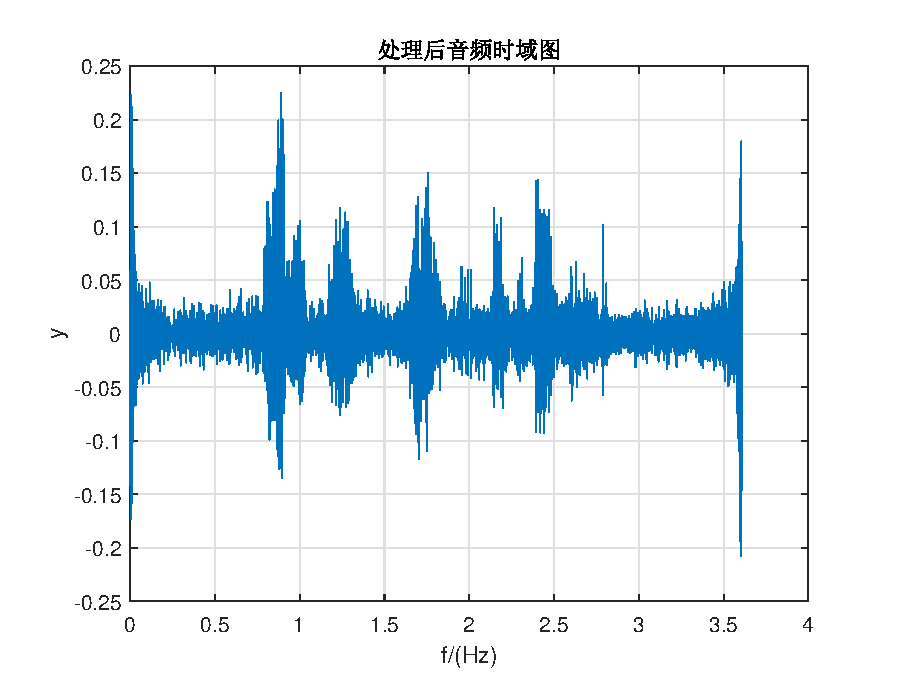
\includegraphics[width=10cm]{112.eps}	
    }
    \caption{双侧音频信号频域域图}
\end{figure}
$\bullet$ 那么可以知道双边频率信号的存在会带来与人声音量相近的持续低噪声,但是会使人声听起来‘更饱和’,于是考虑对双侧信号进行幅度调整减小噪音音量,而非直接滤除。\textit{【此部分噪声在单音噪声之间表现为没有个性的毛刺,故判断此段为宽频噪声,通过资料查询,可以使用幅度调制进行消减】}
\begin{figure}[H]
    \centering
    \
    \subcaptionbox{幅度调整为0.1倍-【频域】}{
        \includegraphics[width=7.2cm]{af-picf0.1.eps}	
    }
    \hfill 
    \subcaptionbox{幅度调整为0.1倍-【时域】}{
        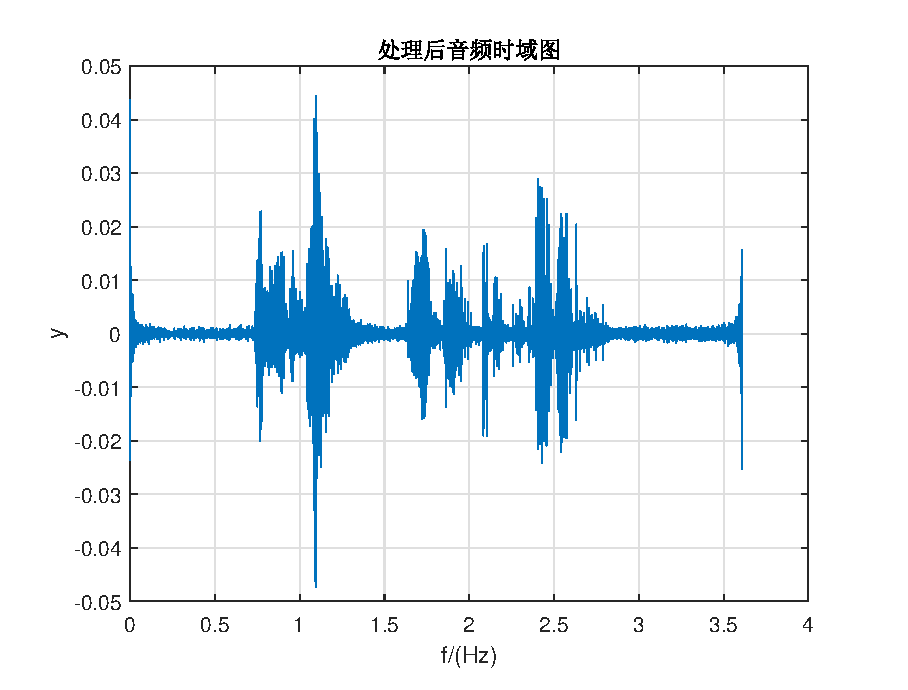
\includegraphics[width=7.2cm]{af-pict0.1.eps}	
    }
    \hfill 
    
    \subcaptionbox{幅度调整为0.5倍-【频域】}{
        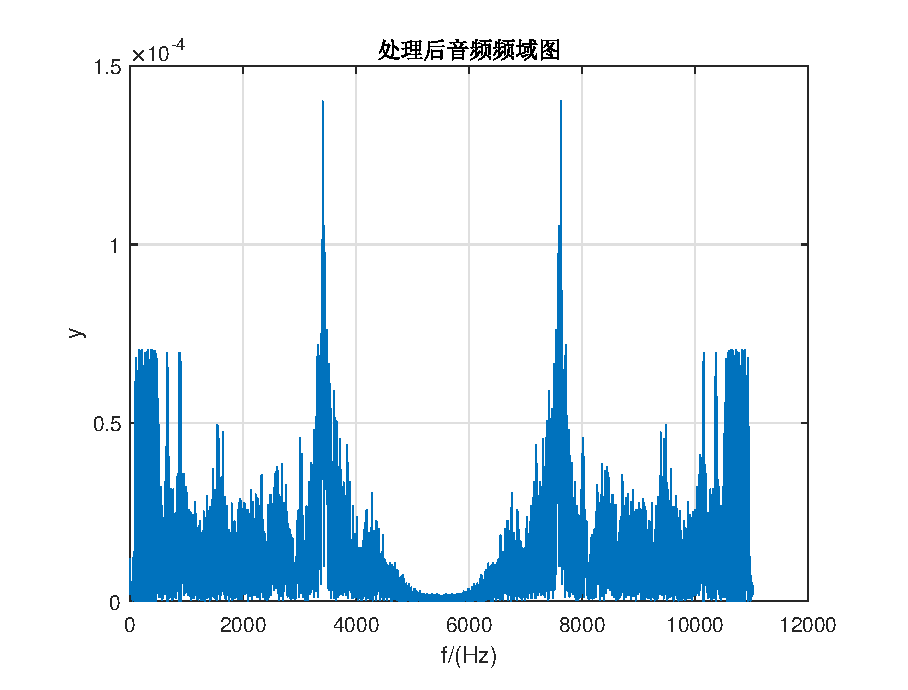
\includegraphics[width=7.2cm]{af-picf0.5.eps}	
    }
    \hfill 
    \subcaptionbox{幅度调整为0.5倍-【时域】}{
        \includegraphics[width=7.2cm]{af-pict0.5.eps}	
    }
    \hfill 
    \subcaptionbox{幅度调整为0.8倍-【频域】}{
        \includegraphics[width=7.2cm]{af-picf0.8.eps}	
    }
    \hfill 
    \subcaptionbox{幅度调整为0.8倍-【时域】}{
        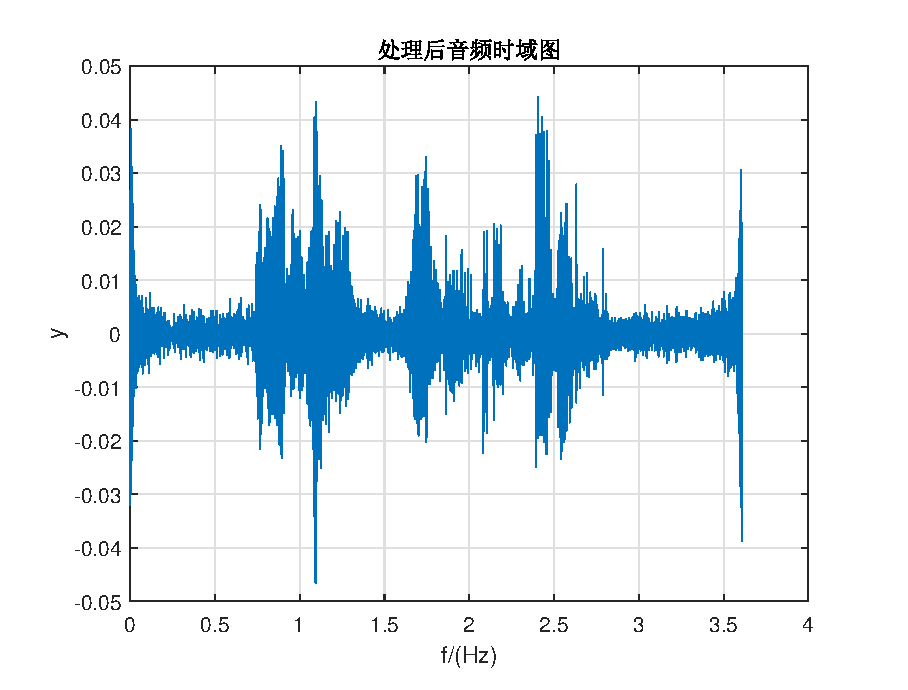
\includegraphics[width=7.2cm]{af-pict0.8.eps}	
    }
    \caption{多次测试-双侧信号幅度调制}
\end{figure} 
$\bullet$ 经过多次尝试,将幅度调整0.2倍时,可以保持人声的‘饱和’同时消减持续低噪声。此时,可认为目前去噪效果呈现为\textbf{最佳状态:可听出音频中男声‘这里是电子科技大学’,且音频噪声较小且人声饱满贴近真实声音}。
\begin{figure}[H]
    \centering
    \subcaptionbox{频域图}{
        \includegraphics[width=11cm]{af-picf0.2.eps}	
    }
    \hfill 
    \subcaptionbox{时域图}{
        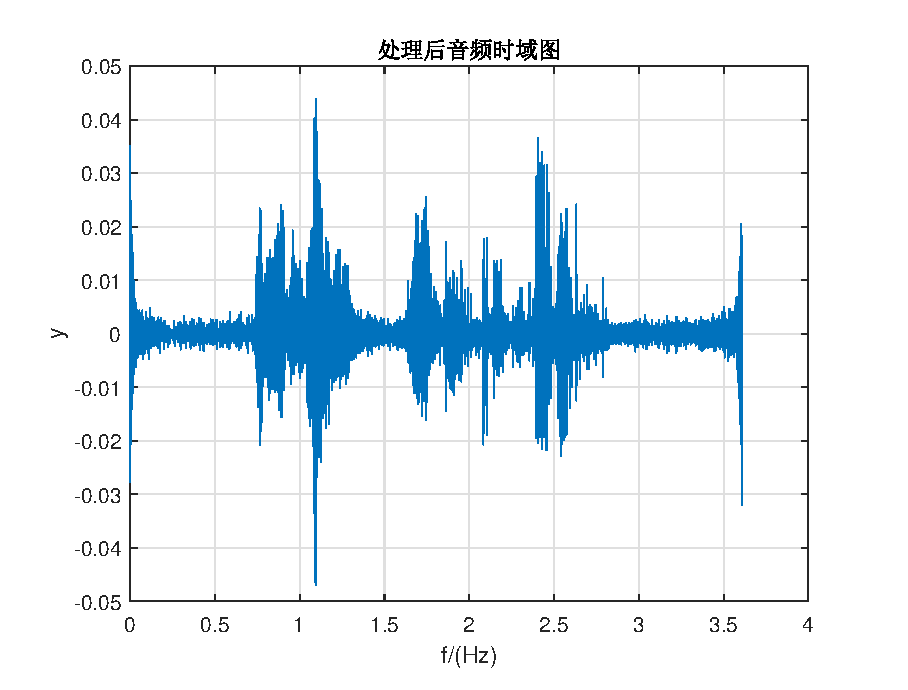
\includegraphics[width=11cm]{af-pict0.2.eps}	
    }
    \caption{最佳处理所得音频信号}
\end{figure}


%\section{设计名称}
去除干扰蜂鸣音
\input{part2}
%\input{part3}
%\input{part4}
\section{实验总结}
这次课程设计的主要原理是利用音频的幅频特性关系在频域将噪音信号去除,主要考察的是信号幅频特性以及滤波器的相关应用。\\
\indent 本设计的去除蜂鸣效果很好,且考虑到低频信号仍包含重要的人声要素,不可使用滤波器直接去除的问题。\textbf{可以将绝大部分的蜂鸣噪音全部去除,并且极高质量地保存了人声语言音频}\textit{【蜂鸣噪声绝大多数被消除且人声语言贴近真实声音、无明显‘失真’】},可以清晰地听到男声语音为:\textbf{“这里是电子科技大学”}。不过在音频开头、结尾仍有一小部分杂音没有去除,这或许是可以进一步改进的地方、但个人判断认为此声音可能是录音开启与结束的操作音直接存在于原始音频中,故而难以被滤除。\\
\indent 同时,本设计的功能相对更加开放,提供了许多可改变参数的参数,故此设计可以面向其他类似的音频使用,具有极大的扩展性。
\input{strengths and weaknesses}
\input{conclusion}
\input{model2}
%\bibliographystyle{plain}
%\bibliography{ref}
\section{附录}
参考资料
\begin{itemize}
    \item [\textbf{1.}] \textit{https://zhuanlan.zhihu.com/p/342854742}
    \item [\textbf{2.}] \textit{https://www.ilovematlab.cn/thread-538265-1-1.html}
    \item [\textbf{3.}] \textit{https://blog.csdn.net/nimentoonaive/article/details/107414105}
\end{itemize} 
%%%%%%%%%%%%%%%%%%%%%%%%%%%%%%
\end{document}
\end